% +++
% latex="texfot lualatex-dev"
% +++
\documentclass[aspectratio=149,10pt,t,]{beamer}
\usetheme[numbering=fraction,block=fill,progressbar=frametitle]{metropolis}
\useoutertheme[right,width=75pt]{sidebar}
\useinnertheme{metropolis}
\usefonttheme{professionalfonts}
\setbeamercolor{frametitle}{use=palette primary,parent=palette primary}

\usepackage{luatexja,luatexja-adjust}
\usepackage[no-math,match]{luatexja-fontspec}
\ltjsetparameter{jacharrange={-2,-8}}

\hypersetup{unicode,colorlinks}
\hypersetup{linkcolor=teal,urlcolor=cyan,citecolor=teal}
% \hypersetup{linkcolor=black,urlcolor=black,citecolor=black}

\usepackage{pxrubrica}
\usepackage{autobreak}
\usepackage{tikz,pgfplots,tcolorbox}
\usetikzlibrary{calc,plotmarks}
\tcbuselibrary{skins}
\pgfplotsset{compat=1.16}

\usepackage{listings}
\lstloadlanguages{TeX}
\lstset{
	doubleletterspace,
	basicstyle={\small\ttfamily},
	%framexleftmargin=5mm,
	frame=shadowbox,
	rulesepcolor=\color{green},
	%numbers=left,
	numberstyle=\tiny,
	morecomment=[l][\rmfamily]{\%},
	columns=fullflexible,
	linewidth=.8\linewidth,
}

\usepackage[version=4,arrows=pgf]{mhchem}
\mhchemoptions{textfontcommand=\sffamily,mathfontcommand=\mathsf}
\newcommand*\cec[1]{\cesplit{{\,\ }{\0}}{#1}}

\usepackage[loadonly,]{enumitem}
\newlist{desc}{description}{5}
\setlist[desc]{labelindent=1\zw,labelsep*=1\zw,labelwidth=3\zw,leftmargin=2\zw}
\newlist{enu}{enumerate}{5}
\setlist[enu]{label*=\arabic*.}

\usepackage{scsnowman} %☃
\usepackage{bxokumacro}
\usepackage{bxwareki}
\usepackage{mflogo}
\usepackage{bxtexlogo}
\bxtexlogoimport{*,**}
\usepackage{tabularray}
\usepackage{efbox}

\usepackage{menukeys}
\renewmenumacro{\keys}[+]{shadowedroundedkeys}
\usepackage{manfnt}

\usepackage{bxrawstr} % https://zrbabbler.hatenablog.com/entry/20181222/1545495849
\usepackage[twemoji-pdf]{bxcoloremoji} % https://github.com/zr-tex8r/BXcoloremoji


% \usepackage[osf]{newpxtext}\usepackage{classico}
\usepackage[nowidering]{yhmath}
\usepackage{newpxmath,amsmath,mathtools,amssymb,mathrsfs,rsfso,mleftright}
\usepackage[T1]{fontenc}
\usepackage[notrig,italicdiff]{physics}
\mleftright

\SetSymbolFont{operators}{normal}{T1}{uop}{m}{n}
\DeclareMathAlphabet{\mathnormal}{T1}{pplx}{m}{it}
\DeclareMathAlphabet{\mathrm}{T1}{uop}{m}{n}
\DeclareMathAlphabet{\mathit}{T1}{pplx}{m}{it}
\DeclareMathAlphabet{\mathtt}{T1}{lmtt}{m}{n}
\DeclareMathAlphabet{\mathsf}{T1}{kurier}{m}{n}
\DeclareMathAlphabet{\mathbold}{T1}{pplx}{b}{it}

\DeclareSymbolFont{numbers}{T1}{pplx}{m}{n}
\DeclareMathSymbol{0}\mathalpha{numbers}{`0}
\DeclareMathSymbol{1}\mathalpha{numbers}{`1}
\DeclareMathSymbol{2}\mathalpha{numbers}{`2}
\DeclareMathSymbol{3}\mathalpha{numbers}{`3}
\DeclareMathSymbol{4}\mathalpha{numbers}{`4}
\DeclareMathSymbol{5}\mathalpha{numbers}{`5}
\DeclareMathSymbol{6}\mathalpha{numbers}{`6}
\DeclareMathSymbol{7}\mathalpha{numbers}{`7}
\DeclareMathSymbol{8}\mathalpha{numbers}{`8}
\DeclareMathSymbol{9}\mathalpha{numbers}{`9}

\DeclareFontFamily{U}{mathastro}{}
\DeclareFontShape{U}{mathastro}{m}{n}{<->mathastrotest10}{}
\DeclareSymbolFont{astro}{U}{mathastro}{m}{n}
\DeclareMathSymbol\Sun\mathord{astro}{'300}
\DeclareMathSymbol\Mercury\mathord{astro}{'301}
\DeclareMathSymbol\Venus\mathord{astro}{'302}
\DeclareMathSymbol\Earth\mathord{astro}{'303}
\DeclareMathSymbol\Mars\mathord{astro}{'304}
\DeclareMathSymbol\Jupiter\mathord{astro}{'305}
\DeclareMathSymbol\Saturn\mathord{astro}{'306}
\DeclareMathSymbol\Uranus\mathord{astro}{'307}
\DeclareMathSymbol\Neptune\mathord{astro}{'310}
\DeclareMathSymbol\Pluto\mathord{astro}{'311}
\DeclareMathSymbol\varEarth\mathord{astro}{'312}
\DeclareMathSymbol\Moon\mathord{astro}{'313}
\DeclareMathSymbol\leftmoon\mathord{astro}{'313}
\DeclareMathSymbol\rightmoon\mathord{astro}{'314}
\DeclareMathSymbol\fullmoon\mathord{astro}{'315}
\DeclareMathSymbol\newmoon\mathord{astro}{'316}
\DeclareMathSymbol\newmoon\mathord{astro}{'316}

\setmainfont[
	Ligatures=TeX,
	Scale=0.98,
	BoldFont=FOT-RodinNTLGPro-B,
	ItalicFont=FOT-RodinNTLGPro-B,
]{Palatino}
\setsansfont[
	Ligatures=TeX,
	Scale=0.98,
	BoldFont=FOT-RodinNTLGPro-B,
	BoldItalicFont=FOT-RodinNTLGPro-B,
	%ItalicFont=FOT-RodinNTLGPro-B,
]{Palatino}
\setmainjfont[
	Ligatures=TeX,
	JFM=jlreq,
	BoldFont=FOT-RodinNTLGPro-B,
	ItalicFont=FOT-RodinNTLGPro-B,
]{FOT-ModeMinBLargePro-M}
\setsansjfont[
	Ligatures=TeX,
	JFM=jlreq,
	BoldFont=FOT-RodinNTLGPro-B,
	ItalicFont=FOT-RodinNTLGPro-B,
]{FOT-ModeMinBLargePro-M}
\setmonofont[
	Ligatures=TeXReset,
]{HackGen}
\setmonojfont[
	Ligatures=TeXReset,
]{HackGen}
\newfontfamily\errorfont[
	Ligatures=TeX,
]{TsukuQMinLStd-L}

\newfontfamily\nishikifonta[
	Ligatures=TeX,
]{Nishiki-teki}
\newjfontfamily\nishikifontj[
	Ligatures=TeX,
]{Nishiki-teki}
\newcommand{\nishikifont}{\nishikifonta\nishikifontj}

\allowdisplaybreaks[4]
\ltjenableadjust[lineend=extended,priority=true,profile=true,linestep=false]

%%%%%%%%%% 以下は自前コマンド

\newcommand{\centeralign}[1]{\rule{0pt}{0pt}\hfill#1\hfill\rule{0pt}{0pt}}
\newcommand{\hmemph}[1]{\textbf{#1}}

\newtcolorbox{typecmdbox}{
	frame engine=empty,
	colback=teal!66!black,
	coltext=lime,
	fontupper=\ttfamily,
	size=small,
	width=.95\linewidth,
}
\newtcbox{typecmd}{
	frame engine=empty,
	colback=teal!66!black,
	coltext=lime,
	fontupper=\ttfamily,
	size=small,
	on line,
}

\newlength{\hmzr}
\newcommand{\hmtexdoc}[1]{
	\settoheight{\hmzr}{\ttfamily ghあ}
	\tikz[baseline=(T.base)]{
		\draw node
		[anchor=south,inner sep=1pt,outer sep=0pt,minimum width=\hmzr,fill=cyan!50!gray,text=white, rotate=90,]
		(T)at(0,0){\resizebox{1.2\hmzr}{.6\height}{texdoc}}
		node
		[anchor=west,inner sep=2pt,outer sep=0pt,signal,minimum height=\hmzr,fill=teal!50!gray,text=lime,font=\ttfamily,]
		(T){#1};
	}
}


\newcommand{\hmunsetap}{
	\metroset{background=light}\usebeamercolor*{normal text}
}
\newcommand{\hmsetap}{
	\metroset{background=dark}\usebeamercolor*{normal text}
}

\newcommand{\hmwaku}[1]{\efbox[margin=0pt]{#1}}

\setlength{\parskip}{1\zw}

\title{最大限 \TeX 入門}
\subtitle{インストールと利用法}
\author{人見祥磨}
\institute{北海道大学理学院 宇宙理学専攻 M2}
\date{\warekitoday}

\begin{document}
\rubyusejghost % \jruby で和文ゴースト
\hmunsetap

\frame[c]{\maketitle}

\begin{frame}
	\frametitle{参考文献}
	\begin{columns}[T]
		\begin{column}{.8\textwidth}
			\begin{itemize}
				\item{}[改訂第 8 版] \LaTeXe 美文書作成入門\\
					{\small (奥村晴彦・黒木祐介 著\quad 技術評論社\textbf{(2020)})}
					\begin{itemize}
						\item 3年毎に改版
						\item 「とりあえずこれを読め」
						\item 網羅的な内容
					\end{itemize}
				\item \LaTeX 超入門 ゼロからはじめる理系の文書作成術\\
					{\small (水谷正大 著 \quad 講談社ブルーバックス\textbf{(2020)})}
					\begin{itemize}
						\item 美文書に比べたら実践的
					\end{itemize}
			\end{itemize}
			{\nishikifont 😀 美文書何章に記述があるか適宜参照します 😀}
		\end{column}
		\begin{column}{.2\textwidth}
			\hmwaku{
\includegraphics[width=.9\textwidth]{bibunsho.jpg}}
			\hmwaku{
\includegraphics[width=.9\textwidth]{chounyumon.jpg}}
		\end{column}
	\end{columns}
\end{frame}

\begin{frame}
	\frametitle{扱うことと扱わないこと}
	\begin{block}{扱うこと}
		\begin{itemize}
			\item \TeX とはなにか
				{\nishikifont\small (美文書 1 章)}
			\item \TeX のインストール方法
				{\nishikifont\small (美文書付録 A 章)}
			\item \TeX の初歩的な使い方
				{\nishikifont\small (美文書 2, 3 章)}
		\end{itemize}
	\end{block}
	\begin{block}{扱わないこと}
		\begin{itemize}
		\item 文書を書くのに使う\jruby[g]{命令}{コマンド}
			{\nishikifont\small (美文書 3, 5--11 章の大半)}
		\item \jruby[g]{命令}{コマンド}の作成
			{\nishikifont\small (美文書 4 章)}
		\item \coloremoji{🍣}\TeX 言語 \coloremoji{🤮}
		\end{itemize}
	\end{block}
\end{frame}

\hmsetap
\begin{frame}
	\frametitle{凡例}
	\begin{itemize}
		\item このスライドのように黒背景のものは内容を飛ばします
		\item 高度な内容なものに関しては \textdbend を付します
		\item \typecmd{緑背景の黄色文字} はターミナルに打ち込むコマンドを示します
	\end{itemize}
\end{frame}

\hmunsetap
\begin{frame}
	\frametitle{目次}
	\setlength{\parskip}{0.5ex}
	\tableofcontents
\end{frame}

\frame[c]{\section{\TeX 概観}{\nishikifont 😀 美文書 1 章 😀}}

\hmunsetap
\begin{frame}
	\frametitle{\protect\TeX でできること、特徴}
	文字を並べた PDF を作ることができる。
	\begin{columns}[T]
		\begin{column}{.5\textwidth}
			\begin{block}{得意なこと}
				\begin{itemize}
					\item きれいな数式
						\[\Pr[d=n]=\log_{10}\left[\frac{n+1}{n}\right]\]
					\item 相互参照、処理の自動化
					\item 様々な OS で利用可能
					\item 実体はテキストファイル\\
						{\scriptsize 計算機で扱いやすい}
				\end{itemize}
			\end{block}
		\end{column}
		\begin{column}{.5\textwidth}
			\begin{block}{できないこと}
				\begin{itemize}
					\item 見たまま編集
					\item 図の描画\\
						{\scriptsize \TikZ などで描画はできる}
					\item フォントを自在に扱う\\
						{\scriptsize 最近は扱いやすくなっている}
				\end{itemize}
			\end{block}
		\end{column}
	\end{columns}
\end{frame}

\begin{frame}
	\frametitle{\TeX, \LaTeX とは何か}
	\begin{block}{\TeX とはなにか}
		\begin{itemize}
			\item 1978 年に Donald E. Knuth が発表した組版システム
				\begin{itemize}
					\item 組版するための\hmemph{ソフトウェア}
					\item 組版するための\hmemph{プログラミング言語}
					\item 相当に古い
				\end{itemize}
		\end{itemize}
	\end{block}
	\begin{block}{\LaTeX とはなにか}
		\begin{itemize}
			\item \TeX を利用して作られたマクロ体系(フォーマット)
			\item \TeX とは別物
		\end{itemize}
	\end{block}
\end{frame}

\begin{frame}
	\frametitle{ナントカ\TeX}
	\begin{block}{\TeX の仲間にはたくさんある(ナントカ\TeX )}
		\begin{desc}
			\item[処理系(エンジン)] \TeX (ソフトウェア)を拡張したもの\\
				\eTeX, \pdfTeX, \XeTeX, \LuaTeX, \pTeX, \upTeX など
			\item[フォーマット] マクロ体系……
				\LaTeX, plain \TeX, \ConTeXt など
		\end{desc}
		全部まとめて\TeX と呼ぶことも多い
	\end{block}
	\begin{block}{よく使うナントカ\TeX}
		\begin{desc}
			\item[\pTeX] 日本語に対応した \TeX エンジン
			\item[\pLaTeX] \pTeX で動く \LaTeX
			\item[up\LaTeXTeX] Unicode に対応した \LaTeXTeX
			\item[Lua\LaTeXTeX] Lua 言語を取り込んだ次世代の \LaTeXTeX
		\end{desc}
	\end{block}
\end{frame}

\begin{frame}
	\frametitle{\TeX の配布}
	\TeX はフリーなソフトで、誰でも入手することができる
	\begin{block}{CTAN (The Comprehensive \TeX Archive Network)}
		\TeX に関する成果物は、CTAN に集められる
		\begin{itemize}
			\item \url{https://www.ctan.org}
			\item ボランティアで成り立っている
		\end{itemize}
	\end{block}
	\begin{block}{\TeX ディストリビューション}
		CTAN から様々なディストリビューション(配布元)へ
		\begin{itemize}
			\item {\TeX} Live (\url{http://www.tug.org/texlive/})
			\item MiK{\TeX} (\url{https://miktex.org})
		\end{itemize}
	\end{block}
\end{frame}

\begin{frame}
	\frametitle{\TeX ディストリビューション}
	\TeX 本体やパッケージ以外にも、関連するバイナリも収録されている
	\begin{block}{texdoc}
		ドキュメントを検索するコマンド texdoc も収録されている
		\begin{typecmdbox}
			texdoc ⟨keyword⟩
		\end{typecmdbox}
		\begin{desc}
			\item[\typecmd{texdoc platex}] \pLaTeX の説明文書
			\item[\typecmd{texdoc platexsheet-jsclasses}] コマンド一覧
		\end{desc}
		スライド中では \hmtexdoc{texdoc} と参照先を示す
	\end{block}
\end{frame}

\hmunsetap
\begin{frame}
	\frametitle{{\TeX} Live \hmtexdoc{texlive}}
	最も普及している \TeX ディストリビューション
	
	膨大な数のパッケージやバイナリが含まれる
	
	晩春に名前が変わる大型アップデート\\
	{\footnotesize 2 月頃に更新停止 (frozen)・次年度版の pretest\\
	2021 年 4 月 1 日~\TeX\ Live 2020 → \TeX\ Live 2021}
	
	バイナリの更新は原則\hmemph{大型アップデート時のみ}\\
	{\footnotesize パッケージ(テキストファイル)の更新は frozen 時以外はいつでも}
	
	大型アップデート時はインストールし直す必要
\end{frame}

\frame[c]{\section{\TeX のインストール} {\nishikifont 🖳 美文書 付録 A 🖳}}

\begin{frame}
	\frametitle{\TeX\ Liveのインストール \hmtexdoc{texlive}}
	詳しくは \TeX\ Wiki~\url{https://texwiki.texjp.org}\\
	または \url{http://www.circle9.work/tex/install.html}\\
	\url{http://www.tug.org/texlive/quickinstall.html}
	
	ネットワーク経由で大量のファイルをダウンロードすることになるので、
	時間があるときに、通信環境がよいところで
	
	\begin{block}{W32\TeX}
		Windows で一般的だったが\hmemph{配布が終了した} (2021/07/13)
	\end{block}
	\begin{block}{MacTeX}
		Mac で一般的だが、様々なバイナリをいろいろな場所に配置するので注意
	\end{block}
\end{frame}

\begin{frame}
	\frametitle{最新の {\TeX} Live をインストールする---UNIX 系の場合}
	TUG (\TeX\ User Group) からインストーラをダウンロード\\
	\url{ftp://ftp.tug.org/texlive/tlnet/}
	\begin{typecmdbox}
		{\scriptsize wget http://mirror.ctan.org/systems/texlive/tlnet/install-tl-unix.tar.gz}
	\end{typecmdbox}
	インストーラを起動してインストール
	\begin{typecmdbox}
		{\scriptsize sudo ./install-tl -no-gui \textbackslash\\
		~~~~-repository http://mirror.ctan.org/systems/texlive/tlnet}
	\end{typecmdbox}
	
	パスを忘れずに通す
	\begin{typecmdbox}
		\scriptsize sudo /usr/local/texlive/????/bin/*/tlmgr path add
	\end{typecmdbox}
	{\scriptsize \typecmd{tlmgr path add} はパスを通すために \TeX\ Live が用意したコマンド}
\end{frame}

\begin{frame}
	\frametitle{{\TeX} Live のアップデート}
	({\TeX} Live をインストールした場合)
	
	\begin{typecmdbox}
		sudo tlmgr update --self --all
	\end{typecmdbox}
	
	上のコマンドで {\TeX} Live をアップデート
	
	定期的にやろう
	
	年度が変わる大型アップデート時には\hmemph{再インストール}
	
	古い \TeX\ 環境がインストールされたまま上からインストールができる\\
	{\small 年度ごとに新しくディレクトリを作成してインストールするため}
\end{frame}

\begin{frame}
	\frametitle{apt でインストールする}
	\begin{typecmdbox}
		sudo apt install texlive-full
	\end{typecmdbox}
	
	apt でもインストール可能
	
	\begin{itemize}
		\item 統一的な管理ができる
		\item tlmgr が使えない
		\item 更新が遅れる
	\end{itemize}
	
	個人的には install-tl でのインストールを勧めたい
\end{frame}

\frame[c]{\section{\TeX の使い方} {\nishikifont 😀 美文書 2 章 😀}}

\begin{frame}
	\frametitle{\TeX で PDF を作成する流れ}
	\begin{columns}[T]
		\begin{column}{0.4\textwidth}
			\centering
			\begin{tikzpicture}[x=.8cm,y=.8cm]
				\node[draw](tex)at(0,0){.tex ファイル};
				\node[draw](dvi)at(0,-2){.dvi ファイル};
				\node[draw](pdf)at(0,-4){.pdf ファイル};
				\draw[->,very thick](tex)--(dvi)--(pdf);
				\coordinate(A)at(0,-1);
				\coordinate(B)at(0,-3);
				\node[right](T)at(0.5,-1){\TeX 処理系};
				\node[right](D)at(0.5,-3){dvi ウェア};
				\draw[<-](A)--(T);\draw[<-](B)--(D);
			\end{tikzpicture}\\
			レガシーな処理系\\
			\pLaTeX, \upLaTeX など
		\end{column}
		\begin{column}{0.4\textwidth}
			\centering
			\begin{tikzpicture}[x=.8cm,y=.8cm]
				\node[draw](tex)at(0,0){.tex ファイル};
				\node[draw](pdf)at(0,-4){.pdf ファイル};
				\draw[->,very thick](tex)--(pdf);
				\coordinate(A)at(0,-2);
				\node[right](T)at(0.5,-2){\TeX 処理系};
				\draw[<-](A)--(T);
			\end{tikzpicture}\\
			モダンな処理系\\
			\LuaLaTeX, \pdfLaTeX など
		\end{column}
	\end{columns}
	\begin{desc}
		\item[\TeX 処理系] 文字の座標を決める
		\item[dvi ウェア] 実際に文字を配置する
		\end{desc}
\end{frame}

\begin{frame}
	\frametitle{dvi ファイル・dvi ウェア}
	\begin{desc}
		\item[dvi] \textbf{D}e\textbf{v}ice \textbf{I}ndependent (装置非依存)の略
		\item[dvi ファイル] どの座標にどの文字を置くのかなどの情報が格納されている
		\item[dvi ウェア] dvi ファイルを変換するソフトウェア
			\begin{itemize}
				\item dvipdfmx(PDF に変換)
				\item dvips(PostScript に変換)
			\end{itemize}
	\end{desc}
	\begin{block}{dvi の仕様}
		\begin{description}
			\item[標準仕様] 装置非依存な部分。dvi ウェアで共通。
			\item[拡張仕様] 装置依存な部分\footnote{色とか用紙サイズとか}。
				dvi ウェアごとに\hmemph{異なる}。
		\end{description}
	\end{block}
\end{frame}

\begin{frame}
	\frametitle{\TeX ソースを書くうえでの注意点}
	使う\TeX 処理系、dvi ウェアによって書き方が微妙に違う
	
	\hmemph{どの処理系、どの dvi ウェアを利用するか気に留める必要}
	
	\begin{block}{日本で一般的な方法}
		\begin{itemize}
			\item {\pLaTeX} + dvipdfmx \hmemph{(古い)}
			\item {\upLaTeX} + dvipdfmx
			\item {\LuaLaTeX}(最近広まりつつある)
		\end{itemize}
	\end{block}
	
	以下、主に {\pLaTeX} + dvipdfmx を例にして話す
	\footnote{\LuaLaTeX は (u)p\LaTeX と書き方がそれなりに異なるので注意}
\end{frame}

\frame[c]{\section{\LaTeX の書き方}{\nishikifont 🤓美文書 3 章🤓}}

\begin{frame}[fragile]
	\frametitle{\LaTeX 文書の作り方}
	\lstinputlisting[caption={sample.tex}]{sample.tex}
	
	BOM なし UTF-8 で保存しましょう
\end{frame}

\begin{frame}
	\frametitle{\LaTeX 文書の作り方}
	\begin{columns}[c]
		\begin{column}{0.5\textwidth}
			コマンドラインで以下を実行
			
			\begin{typecmdbox}
				platex sample\\
				dvipdfmx sample
			\end{typecmdbox}
		\end{column}
		\begin{column}{0.4\textwidth}
			\fbox{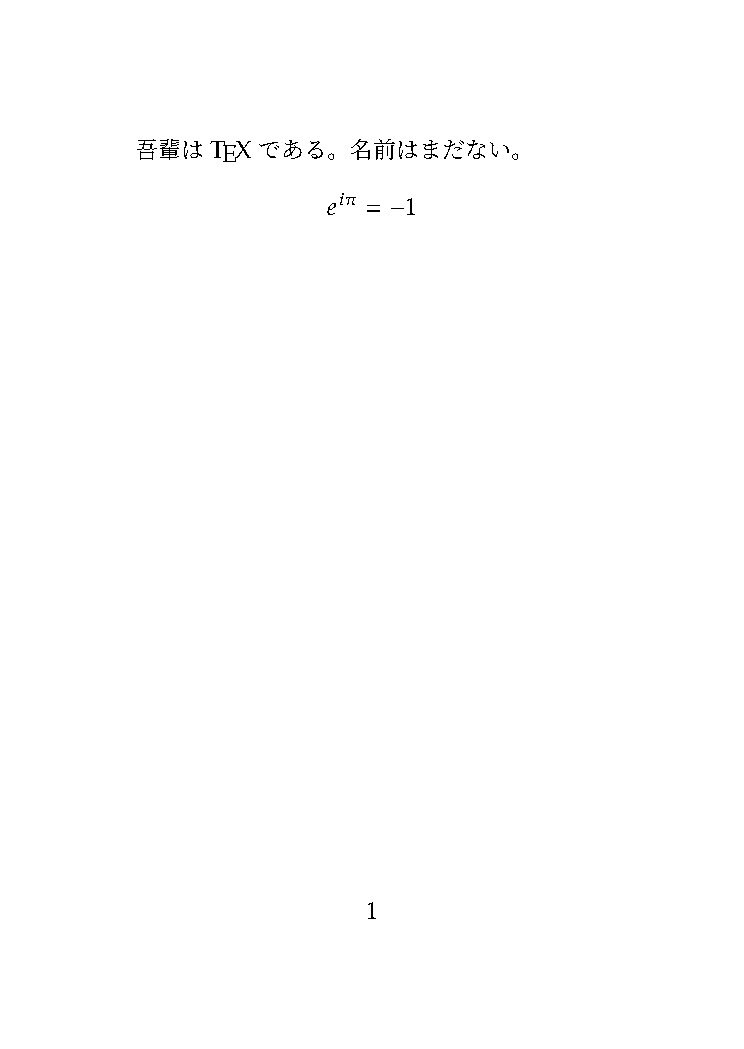
\includegraphics[width=\textwidth]{sample.pdf}}
		\end{column}
	\end{columns}
\end{frame}

\rawstrenable
\begin{frame}[fragile]
	\frametitle{\LaTeX 文書の構造}
	\begin{description}
		\item[{\jruby[g]{命令}{コマンド}}] \texttt{\textbackslash} で始まる、英文字(と和文文字)の列\\
			もしくは \texttt{\textbackslash} のあとに数字か記号ひとつ\\
			\fbox{\texttt{[[|\TeX|]]}} や \fbox{\texttt{[[|\^|]]}} など
			(\jruby[g]{制御語}{コントロールワード}と\jruby[g]{制御文字}{コントロールシンボル})
		\item[環境] \verb+\begin{ナントカ}+ と \verb+\end{ナントカ}+で囲まれたもの
		\item[コメント] \texttt{\%} から行末まではコメント扱い(無視される)
	\end{description}
	
	\begin{block}{特殊な文字}
		以下の文字は特殊文字
		\begin{center}
			\verb+% \ ^ _ ~ { } # & $+
		\end{center}
	\end{block}
\end{frame}
\rawstrdisable

\begin{frame}[fragile]
	\frametitle{\jruby[g]{命令}{コマンド}についての注意}
	\begin{itemize}
		\item \jruby[g]{命令}{コマンド}の引数は \verb+{ }+ で括る
		\item オプショナルな引数は \verb+[ ]+ で括る
	\end{itemize}
	
	\verb+{ }+ はカッコの対応を確認されるが、\\
	{\em\verb+[ ]+ はカッコの対応を確認しない}
	
	例:\\
	\verb+\lstinputlisting[caption=[1]]{foo.tex}+ は\\
	{\em\verb+caption=[1+ だけが \verb+[ ]+ に入っている}判定\\
	→ {\em\verb+[ ]+ に含めたい全体を \verb+{ }+ で括る}と解決\\
	{\footnotesize\verb+\lstinputlisting[{caption=[1]}]{foo.tex}+}
\end{frame}

\begin{frame}[fragile]
	\frametitle{\LaTeX 文書の構造}
	\lstinputlisting{struct.tex}
\end{frame}

\begin{frame}[fragile]
	\frametitle{\LaTeX 文書の構造(ドキュメントクラス)}
	\begin{center}
		\verb+\documentclass[dvipdfmx]{jsarticle}+
	\end{center}
	
	クラスファイルを読み込む→版面構成の定義など\\
	{\footnotesize 実体は ナントカ.cls というテキストファイル}
	
	\begin{block}{主要なクラスファイル}
		\begin{itemize}
			\footnotesize
			\item jsarticle, jsreport, jsbook (新ドキュメントクラス)\\
			\item jlreq(日本語組版処理の要件\footnote{\url{https://www.w3.org/TR/jlreq/ja/}}対応)\\
			\item beamer(スライド用 日本語するには工夫が必要)
			\item jarticle, jreport, jbook(s なし)は\hmemph{非推奨}
		\end{itemize}
	\end{block}
\end{frame}

\begin{frame}[fragile]
	\frametitle{\LaTeX 文書の構造(ドキュメントクラス)}
	\begin{center}
		\verb+\documentclass[dvipdfmx]{jsarticle}+
	\end{center}
	
	[ ] の中はオプション設定\\
	\bgroup\footnotesize フォントサイズ、見開きの設定など
	\begin{center}
		\verb+\documentclass[12pt,dvipdfmx]{jsarticle}+
	\end{center}
	\egroup
	
	\hmemph{必ず}使う dvi ウェアをオプションに設定する\\
	(ドライバオプション)
	\footnote{dvi 拡張仕様の命令を dvi ファイルに埋め込む必要があるため}
\end{frame}

\begin{frame}[fragile]
	\frametitle{\LaTeX 文書の構造(文書本体)}
	\begin{center}
		\verb+\begin{document}+\\
		$\vdots$\\
		\verb+\end{document}+
	\end{center}
	
	文書本体は \verb+\begin{document}+ と \verb+\end{document}+ の間に書く
	
	打ち込んだ文字がそのまま出力される(特殊文字は除く)
	
	\jruby[g]{命令}{コマンド}を利用できる
\end{frame}

\begin{frame}[fragile]
	\frametitle{文書を書くときの注意}
	\begin{block}{改行の扱い}
		\begin{itemize}
			\item 改行は空白扱い
			\item 和文文字直後の改行は無視(空白にもならない)
			\item 連続した改行→改段落
			\item \verb+%+ は改行文字も含めて、行末まで無視する\\
				→空白は入らない
		\end{itemize}
	\end{block}
	
	メール的なフォーマットで書ける\\
	{\footnotesize 1行が長くなったら改行、改段落は空行}
\end{frame}

\begin{frame}[fragile]
	\frametitle{文書を書くときの注意}
	\begin{block}{\jruby[g]{制御綴}{コントロールシークエンス}や空白の扱い}
		\begin{itemize}
			\item 空白はいくつつなげても 1 つに吸収される
			\item 行頭行末の空白は無視される
			\item \verb*+\ + や \verb+~+ で空白を出力できる(\verb+~+ は行分割されない)
			\item \jruby[g]{制御語}{コントロールワード}直後の空白は
				\hmemph{\jruby[g]{制御語}{コントロールワード}の区切りでしかない}\\
				→\hmemph{無視される}
			\item \jruby[g]{制御文字}{コントロールシンボル}直後の空白は\hmemph{無視されない}
		\end{itemize}
	\end{block}
	
	\bgroup\scriptsize
	\begin{tabular}{lclclcl}
		\verb*+\TeX Live+&→&\TeX Live&\hspace*{3em}&\verb*+\TeX  Live+&→&\TeX  Live\\
		\verb*+\TeX\ Live+&→&\TeX\ Live&&\verb*+{\TeX} Live+&→&{\TeX} Live\\
		\verb*+A \& B+&→&A \& B&&\verb*+A\&B+&→&A\&B
	\end{tabular}
	\egroup
\end{frame}

\begin{frame}
	\frametitle{文書を書くときの注意}
	その他の注意、使える命令、環境は
	\begin{itemize}
		\item \typecmd{texdoc platexsheet-jsclasses}
		\item 美文書作成入門
	\end{itemize}
	を参照
	
	\hmemph{ググるより先に上を読みましょう}\\
	{\footnotesize ググって出てくる情報は軒並み古くて怪しい
	\footnote{ディスプレイ数式を \texttt{\$\$ 〜 \$\$} で囲んだり、
	\texttt{\textbackslash begin\{eqnarry\}}を使ったり}}
\end{frame}

\begin{frame}[fragile]
	\frametitle{\LaTeX 文書の構造(プリアンブル)}
	\verb+\documentclass+ から \verb+\begin{document}+ の間\\
	→ \hmemph{プリアンブル (preamble)}
	
	パッケージの読み込み・文書全体の設定をする\\
	{\footnotesize\verb+\usepackage[a4paper]{geometry}+\\
	→ geometry パッケージを、a4paper オプション付きで読み込む}
	
	本文を書くことはできない
	
	逆に、プリアンブルでしか使えないコマンドもある\\
	{\footnotesize \verb+\usepackage+ など}
\end{frame}

\begin{frame}[fragile]
	\frametitle{パッケージとは}
	様々な便利機能を提供\\
	{\footnotesize 他のプログラミング言語で言うところのライブラリ}
	
	実体は、ナントカ.sty というテキストファイル
	
	例: ゆきだるま☃を書きたい!\\
	→ scsnowman パッケージ\\
	→ \verb+\usepackage{scsnowman}+ \\
	→ \verb+\scsnowman[scale=3,hat,arms,buttons]+ \\
	→\scsnowman[scale=3,hat,arms,buttons] 素敵!
\end{frame}

\begin{frame}[fragile]
	\frametitle{パッケージの使い方}
	\begin{enumerate}
		\item 用途からパッケージを探す\\
			{\footnotesize ググるしかない もしくは CTAN でググる
			\footnote{英語なので厳しい; {\tiny ググるを誤用してるのは承知です}}}
		\item プリアンブルで\\\verb+\usepackage[オプション]{パッケージ名}+
		\item 使う
		\item 使い方がわからなくなるので \typecmd{texdoc パッケージ名}
	\end{enumerate}
\end{frame}

\begin{frame}[fragile]
	\frametitle{おすすめプリアンブル}
	\begin{center}
		\lstinputlisting[basicstyle=\ttfamily\scriptsize]{preamble.tex}
	\end{center}
	
	\LaTeX を理解するまでは、これをそのまま使おう
\end{frame}

\begin{frame}[fragile]
	\frametitle{書き方まとめ}
	\lstinputlisting{sample2.tex}
\end{frame}

\begin{frame}[fragile]
	\frametitle{(u)p{\LaTeX} VS \LuaLaTeX}
	\lstinputlisting[basicstyle=\ttfamily\tiny,caption={sample-lualatex.tex}]{sample-l.tex}
	
	\begin{block}{\LuaLaTeX を利用する場合}
		\begin{itemize}
			\scriptsize
			\item jsclasses は \pLaTeX 専用 → ltjsclasses
			\item ドライバオプションは不要
			\item フォントの世話: fontenc → fontspec
			\item otf パッケージも \pLaTeX 専用 → 削除
		\end{itemize}
	\end{block}
\end{frame}

\frame[c]{\section{エラーへの対処}{\nishikifont 😱美文書 2 章 9 節😱}}

\begin{frame}
	\centering\nishikifont
	\frametitle{\coloremoji{⚠️}ご注意ください\coloremoji{⚠️}}
	\centering\LARGE
	😱😱😱😱😱😱😱😱😱😱
	
	エラー対処が上手かどうかで\\
	作業効率が激変します
	
	😱😱😱😱😱😱😱😱😱😱
\end{frame}

\begin{frame}[fragile]
	\frametitle{エラーに遭遇する}
	\TeX は\hmemph{プログラミング言語}\\
	書き方を間違えるとエラーが出る
	
	\verb+\TEX+ と書いてしまうと……
	
	\bgroup\errorfont
	\begin{tabbing}
		! Undefined control sequence.\\
		l.3 \verb+\TEX+\\
	\end{tabbing}
	\egroup
	「{\errorfont ?}」と聞かれるので、\keys{X} \keys{Q} \keys{\return} のどれかを押す
\end{frame}

\begin{frame}
	\frametitle{エラーが出たら}
	\begin{description}
		\item[\keys{X}] 処理を中断して終了
		\item[\keys{Q}] 処理を継続、ログは標準出力しない
		\item[\keys{\return}] 処理を継続、再びエラーが出ると止まる
	\end{description}
	
	\keys{\return} を数回連打するのがおすすめ\\
	{\footnotesize 大抵、複数のエラーが混入しているため}\\
	連続して 5 回以上エラーが出てきたら\keys{X}するべし
\end{frame}

\rawstrenable
\begin{frame}[fragile]
	\frametitle{{\errorfont ?} 以外のプロンプトの場合}
	\begin{block}{\fbox{\errorfont Enter file name:}\\
		{\footnotesize \texttt{[[|\usepackage|]]} でパッケージ名を間違えたときに出がち}}
		
		\keys{X}を押して \keys{\return}
	\end{block}
	\vfill
	\begin{block}{\fbox{\errorfont *}\\
		{\footnotesize \texttt{[[|\end{document}|]]} を忘れたときに出がち}}
		\begin{enumerate}
			\item \verb+\stop+ と打って \keys{\return}
			\item \verb+\aaa+(未定義の\jruby[g]{制御綴}{コントロールシークエンス})
				を打って \keys{\return}\\
				→ {\errorfont ?} のプロンプト → \keys{X}
			\item \keys{\ctrl+C}
		\end{enumerate}
	\end{block}
\end{frame}
\rawstrdisable

\begin{frame}
	\frametitle{エラーメッセージの見方}
	
	\bgroup\errorfont
	\begin{tabbing}
		! You can't use `macro parameter character \#' in horizontal mode.\\
		l.3 O-oooooooooo \#\=\\
		                  \>AAAAE-A-A-I-A-U- \\
		?
	\end{tabbing}
	\egroup
	
	\begin{tabbing}
	! エラーメッセージ\\
	l. 行数~~~\= \TeX が読み込んだもの\=\\
		\>\>まだ読み込んでいないもの
	\end{tabbing}
	
	エラーが出た行に戻って治せばいいのだが……
\end{frame}

\begin{frame}
	\frametitle{エラーへの対処}
	\begin{block}{大体のエラーの原因}
		\begin{itemize}
			\item \jruby[g]{制御綴}{コントロールシークエンス}の綴りのマチガイ
			\item 環境の閉じ忘れ
			\item ものの不均衡(\texttt{\{ \}}、\texttt{\$ \$}%
				\footnote{\texttt{\$ \$} よりも、\texttt{\textbackslash( \textbackslash)}
				を使うほうが好ましいとされます。(「数式組版」(木枝祐介 ラムダノート
				株式会社\textbf{(2018)}))}、
				\texttt{\textbackslash left \textbackslash right} など)
			\item \jruby[g]{命令}{コマンド}の用法のマチガイ
		\end{itemize}
	\end{block}
	
	エラーが起きた行付近で上がないか確認
	
	\jruby[g]{命令}{コマンド}の用法のマチガイ→\typecmd{texdoc <パッケージ名>} で確認
\end{frame}

\begin{frame}
	\frametitle{対処しにくいエラー}
	\begin{block}{おさらい}
		\LaTeX は \TeX のフォーマット(マクロ体系)\\
		→\hmemph{\LaTeX レベルのエラーと、\TeX レベルのエラーがある}
	\end{block}
	起きたエラーによっては、原因が特定しにくい\\
	{\footnotesize 例: {\errorfont ! Missing number, treated as zero.}}
	
	処理中に外部ファイルを読み込むこともある\\
	→行番号が、\hmemph{どのファイルの行番号かわからなくなる}
\end{frame}

\begin{frame}[fragile]
	\frametitle{エラーを起こさないために}
	\begin{itemize}
		\item タイプセットを細かく行う
		\item 開いた環境はすぐ閉じる
		\item 全角空白「 」を使わない\\
			{\footnotesize 段落頭の字下げは \verb+\parindent+ で設定\\
			\tiny 欧文クラスで、一番最初のパラグラフを字下げしたい場合 → indentfirst パッケージ}
		\item \verb+\verb+ 命令もなるべく避ける\\
			{\footnotesize \jruby[g]{命令}{コマンド}の引数にあるとエラー(\verb+\verb+ の呪い)}
	\end{itemize}
	それでも意味不明なエラーが起きる
\end{frame}

\begin{frame}[fragile]
	\frametitle{パッケージの衝突}
	\lstinputlisting[basicstyle=\ttfamily\scriptsize]{error.tex}
	\vspace{-1ex}\centeralign{↓}\vspace{-1ex}
	\bgroup\errorfont\scriptsize
	\begin{tabbing}
		! LaTeX Error: \=Command \verb+\iint+ already defined.\\
		\>Or name \verb+\end+... illegal, see p.192 of the manual.\\
		l.645 ...d\verb+{\iint}{\DOTSI\protect\MultiIntegral{2}}+\\
	\end{tabbing}
	\egroup 	mathabx と ymasth が同じ\jruby[g]{命令}{コマンド}を定義→エラー
\end{frame}

\begin{frame}
	\frametitle{衝突の回避}
	パッケージを読み込む順番を変えたら誤魔化せる場合も\\
	→ 読み込む順番を変えてみる\\
	→ どうしようもなければ諦める
	
	パッケージが日本語対応してなくてエラーが起きる場合も\\
	→ (u)p\LaTeX なら plautopatch パッケージ
	\footnote{\url{https://aminophen.github.io/slide/hytexconf18.pdf}}を試す\\
	→ \LuaLaTeX なら日本語非対応の問題はおこりにくい
\end{frame}

\begin{frame}
	\frametitle{エラーが解消できなくてどうしようもないときは}
	とりあえずエラーメッセージでググってみる\\
	{\tiny これで解決できたら苦労しないんだよなぁ わかりにくいエラーメッセージが嫌ならば、\SATySFi ……?}
	
	わからなければ詳しい人に聞く\\
	{\footnotesize TeX Forum\footnote{\url{https://oku.edu.mie-u.ac.jp/tex/}} で質問\\
	Twitter でつぶやくのも実は有用}
	
	実はバグを踏んでいる可能性も
\end{frame}

\begin{frame}[fragile]
	\frametitle{わかりにくいエラー①}
	
	\verb+[a] 真鍋 \\ [b] いつき+\\
	→{\errorfont ! Missing number, treated as zero.}
	
	\verb+\\+(強制改行)命令は、実はオプション引数をもつ\\
	\hspace*{1em}→\verb+\\[<長さ>]+
	
	\verb+\\{}+ のように \verb+{}+で区切ると解決
	
	\bgroup\footnotesize
	\begin{tabbing}
		\verb+[a] 真鍋 \\{} [b] いつき+\\
		→\=[a] 真鍋 \\{} \> [b] いつき
	\end{tabbing}
	\egroup
\end{frame}

\rawstrenable
\begin{frame}[fragile]
	\frametitle{わかりにくいエラー②}
	
	\verb+\section{$\overrightarrow{\mbox{ぶーん}}$}+\\
	→{\errorfont ! Illegal parameter number in definition of \verb+\reserved@a+.}
	
	エラーが起きる原因→\coloremoji{🤮}
	\footnote{{\ttfamily[[|\section|]]} の引数は動くので、脆弱な 
	{\ttfamily[[|\overrightarrow|]]} は保護しなければならない}
	
	\verb+\section+ や \verb+\caption+ で変なエラーが出たら、\\
	引数に入ってるヤバそうな\jruby[g]{命令}{コマンド}に \verb+\protect+ を前置
	
	{\footnotesize\verb+\section{$\protect\overrightarrow{\mbox{ぶーん}}$}+\\
	→ $\protect\overrightarrow{\mbox{ぶーん}}$}
\end{frame}
\rawstrdisable

\frame[c]{\section{\TeX のディレクトリ構成} {\nishikifont ☃美文書 付録 B 3 節☃}}

\begin{frame}
	\frametitle{TEXMF ツリー}
	\TeX 関連ファイルを入れるディレクトリ構成\\
	{\footnotesize TEXMF ← \TeX + \MF\footnote{\MF は Knuth が作ったフォント記述言語}}
	
	複数の TEXMF ツリーを使い分けるのが主流\\
	\hmemph{多重 TEXMF ツリー}
	
	確認方法: \typecmd{kpsewhich -var-value TEXMF}
\end{frame}

\begin{frame}
	\frametitle{多重 TEXMF ツリーの利点}
	ディストリビューションが用意したファイルと、自分がインストールしたファイルを分離できる
	
	ディストリビューションを更新しても、自分のインストールしたファイルは削除されない
	
	\begin{tabbing}
	\hspace*{3\zw}\=\kill
	ディストリビューションが用意したファイル\\
		\>{→\scriptsize\typecmd{kpsewhich -var-value TEXMFDIST}}\\
	自分がインストールするファイル\\
		\>{→\scriptsize\typecmd{kpsewhich -var-value TEXMFLOCAL}}\hspace{1\zw}\={\scriptsize 全ユーザーが使える}\\
		\>{→\scriptsize\typecmd{kpsewhich -var-value TEXMFHOME}}\>{\scriptsize そのユーザーが使える}
	\end{tabbing}
\end{frame}

%\begin{frame}
%	\frametitle{kpathsea ライブラリ と \aruby{ls-R}{ファイル一覧}}
%	\begin{block}{kpathsea ライブラリ}
%		TEXMF ツリーからファイルを検索する\\
%		{\footnotesize Karl Berry 氏によって作られた path searching}
%		
%		例: \typecmd{kpsehwhich hmtrump.sty}\\
%		{\scriptsize →\texttt{/usr/local/texlive/texmf-local/tex/latex/local/hmtrump.sty}}
%	\end{block}
%	
%	TEXMF ツリーに作られた \aruby{ls-R}{ファイル一覧} を見て検索する\\
%	TEXMF ツリーに変更 → \aruby{ls-R}{ファイル一覧} を更新する必要
%	\footnote{ls-R を使わない運用方法もあるらしいですが、やったことがないのでわかりません}\\
%	\typecmd{sudo mktexlsr}
%\end{frame}

\begin{frame}
	\frametitle{パッケージをインストールする}
	ディストリビューションに含まれないパッケージを使いたい\\
	→自分で TEXMF ツリー \textbf{(TEXMFLOCAL)} に入れる必要\\
	{\footnotesize 作業ディレクトリに置いてもよいけれども}
	
	正しい場所に入れなければ正常に使えない
	\footnote{拡張子に応じて、検索するディレクトリを決め打ってるため}
\end{frame}

\begin{frame}
	\frametitle{TEXMF ツリーの構造}
	TEXMFLOCAL\footnote{{\TeX} Live on UNIX の標準では \texttt{/usr/local/texlive/texmf-local}}
	の構造を覗いてみる
	\footnote{\href{https://texwiki.texjp.org/?TeX\%20\%E3\%81\%AE\%E3\%83\%87\%E3\%82\%A3\%E3\%83\%AC\%E3\%82\%AF\%E3\%83\%88\%E3\%83\%AA\%E6\%A7\%8B\%E6\%88\%90}
	{https://texwiki.texjp.org/?TeX\%20のディレクトリ構成}参照}\\
	\typecmd{tree -d -L 2 /usr/local/texlive/texmf-local}
	
	\begin{columns}
		\begin{column}{0.6\textwidth}
			ファイルの種類ごとに分類
			\begin{description}
				\small
				\item[doc] ドキュメント(説明書)
				\item[tex] パッケージの本体など
				\item[font] フォント関連
			\end{description}
			さらにサブディレクトリで分類\\
			そのなかでパッケージごとに分類
		\end{column}
		\begin{column}{0.35\textwidth}
			\tiny\ttfamily
			/usr/local/texlive/texmf-local\\
			├── doc\\
			│   ├── fonts\\
			│   ├── latex\\
			│   └── lualatex\\
			├── source\\
			│   └── latex\\
			├── tex\\
			│   ├── latex\\
			│   ├── lualatex\\
			│   └── plain\\
			├── texdoc\\
			├── tlpkg\\
			└── web2c
		\end{column}
	\end{columns}
\end{frame}

\begin{frame}
	\frametitle{パッケージをインストールする場所}
	前述の通り、分類して TEXMFLOCAL に配置
	
	まずはパッケージドキュメントを確認
	
	\begin{block}{ドキュメントに記載がない場合: あまり失敗しない方法}
		以下にディレクトリを掘ってファイルを配置
		\begin{itemize}
			\small
			\item ドキュメント→ \texttt{\$TEXMFLOCAL/doc/latex/<pkgname>}
			\item *.dtx, *.doc→ \texttt{\$TEXMFLOCAL/source/latex/<pkgname>}
			\item その他→ \texttt{\$TEXMFLOCAL/tex/latex/<pkgname>}
		\end{itemize}
	\end{block}
	
	フォント関連などはもっと複雑
\end{frame}

\begin{frame}
	\frametitle{参考文献}
	\hmemph{とりあえず美文書は読んでください}
	
	\begin{block}{もっと詳しく知りたい場合}
		\begin{itemize}
			\item {\TeX} Wiki\\\url{https://texwiki.texjp.org}
			\item Acetaminophen'{\kern-0.7em}s diary\\\url{http://acetaminophen.hatenablog.com}
		\end{itemize}
	\end{block}
	
	\bgroup\footnotesize
	\begin{block}{以下のブログは、もっと沼にハマりたい人向け}
		\begin{itemize}
			\item ラングラグー\\\url{https://blog.wtsnjp.com}
			\item マクロツイーター\\\url{https://zrbabbler.hatenablog.com}
		\end{itemize}
	\end{block}
	\egroup
\end{frame}
\end{document}
